The final layer of the ID is a sub-detector called the Transition Radiation Tracker (TRT)~\cite{atlas_trt} which utilizes gas-filled drift tubes for detecting charged particles, unlike the other sub-detectors. The TRT is composed of 300,000 thin-walled drift tubes, often referred to as straws, each filled with a gas mixture of xenon (70\%), $\mathrm{CO}_2$ (27\%) and $\mathrm{O}_2$ (3\%). This choice of gas is no coincidence with xenon being used due to its good X-ray absorption, while the two other gases help increase electron drift velocity, and suppress photon quenching. 

Each straw is 4 mm in diameter with a gold-plated tungsten wire located in the center of the tube that is kept grounded. The exterior of the straw is kept at high voltage with negative polarity creating an electric field between the walls and the wire. When a charged particle passes through a straw, the gas inside the straw ionizes, creating free electrons. The free electrons drift towards the wire because of the voltage differential and produce a signal that is amplified and read out via both ends of the tube.

In addition, the TRT is designed to detect transition radiation photons. When a charged particle traverses the boundary between materials with different dielectric constants, in the case of the TRT these are polymer fibres and foils, soft X-ray photons are produced. These photons are detected in the straws by being absorbed by the xenon atoms which ionize, creating a free electron that drifts to the central wire. Transition radiation is a function of $\gamma$ and is defined as $\gamma = \frac{E}{m}$. Therefore, a light particle, such as an electron, emits a lot more photons than a heavier particle, such as a pion with the same energy. When an excess of energy is deposited in a straw, beyond what is expected for the usual ionizing particles, it is a strong indication that the particle is an electron.
A cross sectional view of the TRT with a particle passing through some straw tubes can be seen in Figure~\ref{fig:atlas_trt_straw_hits}.

\begin{figure}
    \centering
    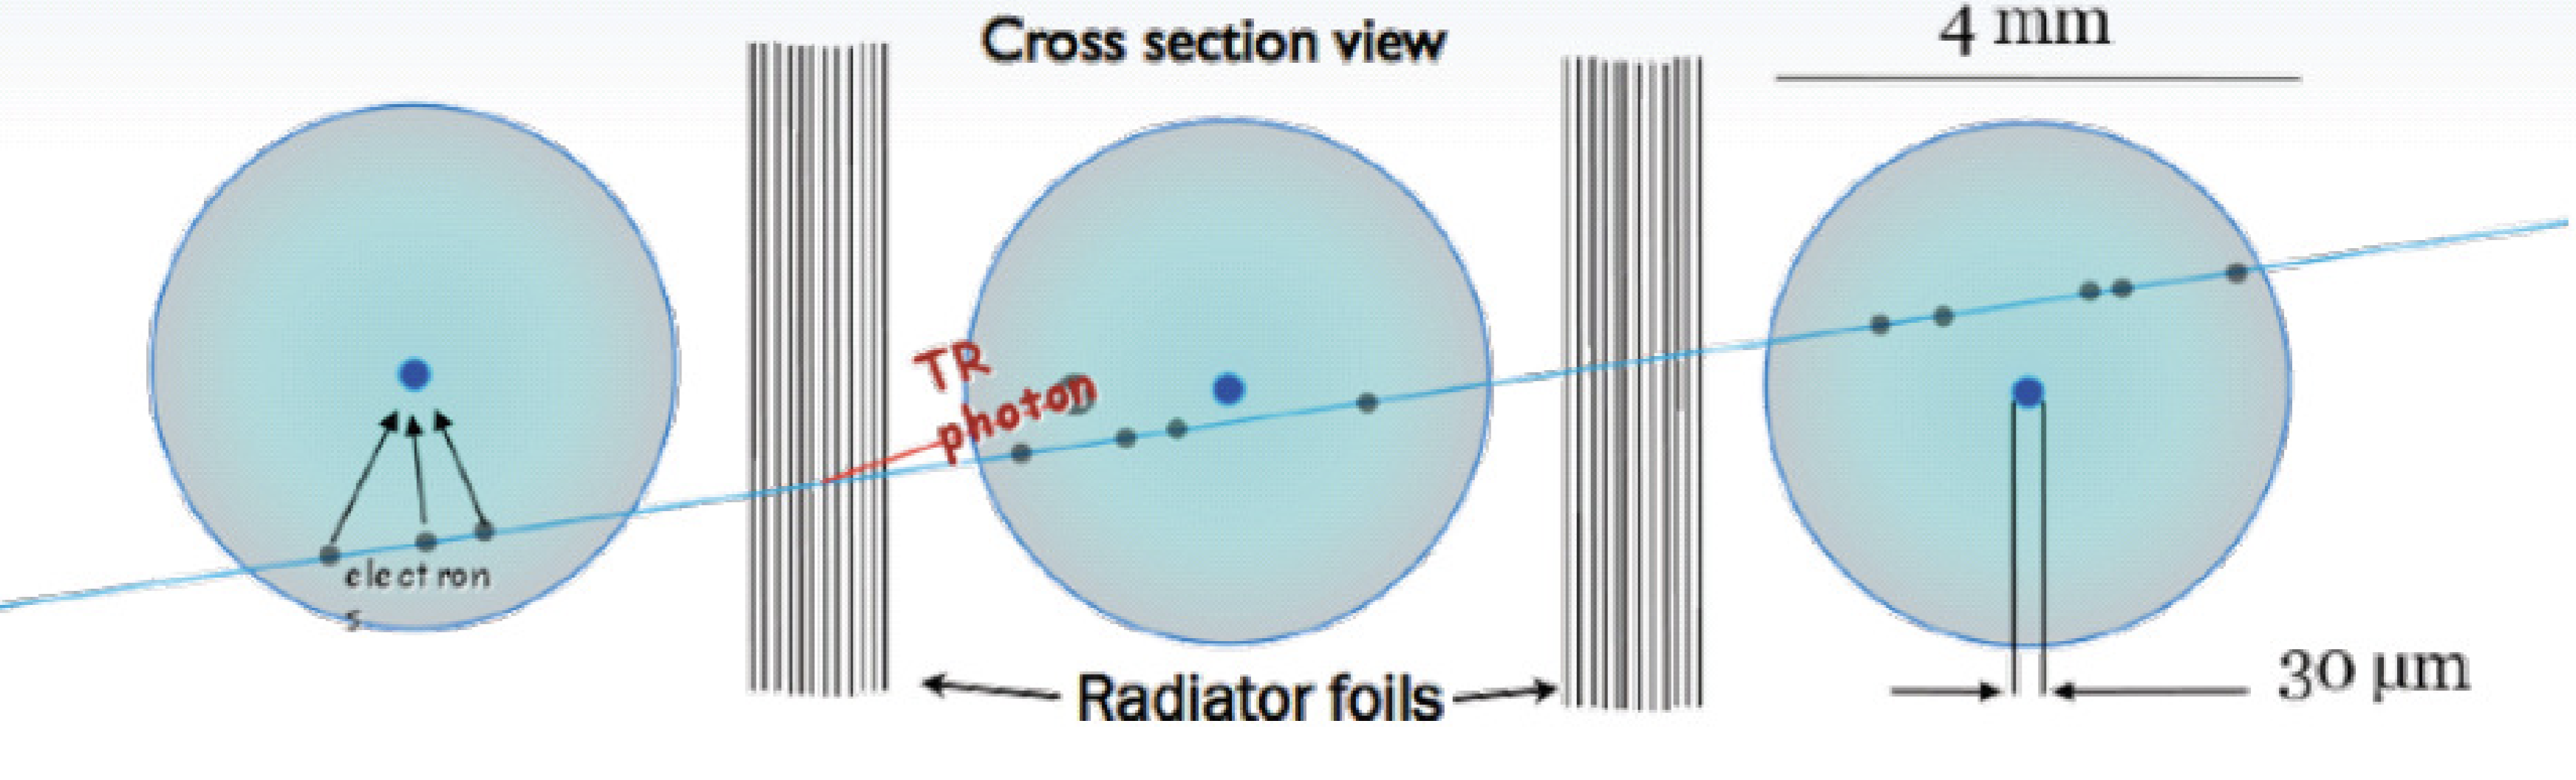
\includegraphics[width=0.8\textwidth]{figures/atlas/atlas_trt_tubes.png}
    \caption{A cross sectional view of the TRT with a particle passing through several straws is depicted. Shown is a particle ionizing the gas at it passes through the straws, creating free electrons. Additionally shown is transition radiation
    that is produce via a particle traversing the foils. Taken from~\cite{atlas_trt}}\label{fig:atlas_trt_straw_hits}
\end{figure}

Similarly to the other sub-detectors, the TRT consists of a barrel and two end-cap regions. The barrel consists of approximately 100,000 straw tubes of length 144 cm, that are laid parallel to the beam axis, arranged in 73 layers, and covers the range of $|\eta| < 1$. In contrast, each end-cap consists of approximately 120,000 straw tubes that are 39 cm in length, oriented in the radial direction, with 160 layers, and covers the range of $1 < |\eta| < 2$. On average, a charged particle is expected to cross 30 straws. The barrel and end-cap schematics can be seen in Figure~\ref{fig:atlas_id} and Figure~\ref{fig:atlas_id_endcap} respectively.